\subsection{Parallel Sum}

Motivations:
\begin{enumerate}
 \item \textbf{technique}: divide-and-conquer
 \item \textbf{pattern}: to solve other associative operations
 \item \textbf{module}: subproblem of other prolems
\end{enumerate}

\textbf{Sequencial sum}\\
\begin{algorithm}[H]
 \SetAlgoLined
 \KwIn{$M[1], M[2], ..., M[n]$}
 \KwResult{$M[n] = \sum_{i=1}^{n}M[i]$}
 \For{$i=1 \ to \ n-1$} {
  $M[n] = M[n] + M[i]$ 
 }
 %\Return{}
 \caption{Sequencial sum ($T(n,1) = n-1$)}
\end{algorithm}

To parallelize this algorithm there are two ways.
\begin{enumerate}
 \item one sum per processor\\
 The heigh of the tree is $n-1$ and the efficiency is $E = \frac{\cancel{n-1}}{\cancel{(n-1)} \cdot (n-1)} \rightarrow 0$
 \item associative sum\\
 The heigh of the tree is $\log{n}$. \\
 This is of course possibile because $((\alpha+\beta)+\gamma)+\delta = (\alpha+\beta)+(\gamma+\delta)$
\end{enumerate}

\textbf{Parallel sum} (using second way)\\
\begin{algorithm}[H]
 \SetAlgoLined
 Let $n = 2^t$ (items to add)
 \KwIn{$M[1], M[2], ..., M[n]$}
 \KwResult{$M[n] = \sum_{i=1}^{n}M[i]$}
 \For{$j=1 \ to \ \log{n}$} {
  \For{$K=1 \ to \ n/2^j$ /*parallelize*/} {
   $M[2^{j}K] = M[2^{j}K] + M[2^{j}K - 2^{j-1}]$ 
  } 
 }
 \Return{$M[n]$}
 \caption{Parallel sum}
\end{algorithm}

\textbf{Instruction}:\\
\textit{1 step}: $M[2K] = M[2K] + M[2K-1] \ || \ 1 \leq K \leq n/2$\\
\textit{2 step}: $M[4K] = M[4K] + M[4K-2] \ || \ 1 \leq K \leq n/4$\\
\textit{3 step}: $M[8K] = M[8K] + M[8K-4] \ || \ 1 \leq K \leq n/8$\\
...\\
\textit{$\log{n}$ step}: $M[n] = M[n] + M[n/2] \ || \ 1$\\

\textbf{Is it EREW?}\\
No, read and write simultaneously in the same cell of M.\\

Processors $a,b \rightarrow a \neq b$ \\
Cells involved by $a$ and $b$:\\
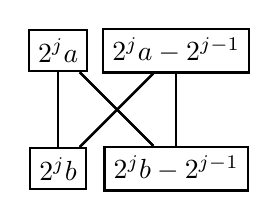
\begin{tikzpicture}[node distance={15mm}, thick, main/.style = {draw}] 
\node[main] (1) {$2^{j}a$}; 

\node[main] (2) [right of=1] {$2^{j}a - 2^{j-1}$}; 
\node[main] (3) [below of=1] {$2^{j}b$}; 
\node[main] (4) [right of=3] {$2^{j}b - 2^{j-1}$};

\draw (1) -- (3);
\draw (1) -- (4);
\draw (2) -- (3);
\draw (2) -- (4);

\draw (3) -- (1);
\draw (3) -- (2);s
\draw (4) -- (1);
\draw (4) -- (2);

\end{tikzpicture} 

\textbf{Comparisons}:\\
$2^{j}a \neq 2^{j}b$ yes, for $a \neq b$\\
$2^{j}a \neq 2^{j}b - 2^{j-1}$ $\overset{by \ contradiction}{\Rightarrow}$ $2a = 2b - 1 \Rightarrow a = \frac{2b-1}{2} \notin \mathbb{N}$\\
!!! EREW algorithm

\begin{proof}
$M[2^{j}K] = M[2^{j}K] + \dots + M[2^{j}(K-1)+1]$\\
Per $j=log{n}$, obviously $K=1$ e we have that:\\
$M[n] = M[n] + \dots + M[1]$.\\
Proof by induction:\\
\textit{Base case:} $j=1$ and $1 \leq K \leq n/2$	\\
Algorithm instruction: $M[2K] = M[2K] + \dots + M[2K-1]$.\\
END.
\end{proof}

